\subsection{Winkelrichtgröße}
Die Winkelrichtgröße berechnet sich durch
\begin{equation}
  D = \frac{F\cdot r}{\phi}.
\label{eqn:WRG}
\end{equation}
Diese Rechnung wird für alle gemessenenen Winkel $\phi$ und dazugehörigen Kräfte F ausgeführt.
Die Werte sind in Tabelle \ref{tab:WRG} zu finden.
\begin{table}[h!]
  \centering
  \caption{Messdaten zur Bestimmung der Winkelrichtgröße}
  \label{tab:WRG}
  \begin{tabular}{c c c c}
    \toprule
     $\phi/°$ & $\phi/rad$  &  $F/N$	&  $D/Nm$     \\
    \midrule
      \input{Winkelrichtgröße.txt}
    \bottomrule
  \end{tabular}
\end{table}

\\Allgemein wird ein Mittelwert über folgende Formel ermittelt:
\begin{equation}
  \mu = \frac{1}{N} \sum_{n=1}^{N} x_{n}.
\label{eqn:mw}
\end{equation}
\\Dabei ist N die Anzahl der Werte und $x_{n}$ sind die Werte.
\\Die dazugehörige Standardabweichung wird durch
\begin{equation}
  \sigma =  \sqrt{  \frac{1}{N-1}  \sum_{n=1}^{N} (x_{n} - \mu)^2 }
\label{eqn:sigma}
\end{equation}
\\errechnet.
\\Die zehn Werte der Winkelrichtgröße in Tabelle \ref{tab:WRG} werden gemittelt.
Es ergibt sich der verwendete Wert der Winkelrichtgröße D
\begin{equation*}
  D = \SI{0.0200 \pm 0.0018}{Nm}.
\end{equation*}

\subsection{Eigenträgheitsmoment}
Für das Eigenträgheitsmoment werden die Schwingungsdauern der Konstruktion und die Abstände der beiden Massen $m_{ID}=0.2218$ kg zur Drehachse bei dem Winkel $\phi = 180°$ aufgetragen und jeweils quadriert (Tabelle \ref{tab:ETM}).
Die beiden Zylinder haben die Höhe $h_{ID}=0.0296$ m und den Radius $r_{ID}=0.1745$ m.
\begin{table}[h!]
  \centering
  \caption{Messdaten zur Bestimmung des Eigenträgheitsmomentes}
  \label{tab:ETM}
  \begin{tabular}{c c c c}
    \toprule
     $a/m$ &  $a^2/m^2$	 &  $T/\frac{1}{s}$ & $T^2/\frac{1}{s^2}$ \\
    \midrule
      \input{Eigenträgheitsmoment.txt}
    \bottomrule
  \end{tabular}
\end{table}

\\Das Eigenträgheitsmoment setzt sich aus verschiedenen Formeln zusammen.
\\Das Gesamtträgheitsmoment zweier gleicher Zylinder, die im gleichen Abstand zur selben Drehachse stehen, lautet nach Formel \eqref{eqn:steiner} und Formel \eqref{eqn:Zl}:
\begin{equation*}
  I_{2z, liegend} = I_{D} + 2 \cdot m_{ID} \cdot \left(\frac{r_{ID}^2}{4} + \frac{h_{ID}^2}{12} \right) + 2 \cdot m_{ID} \cdot a_{ID}^2.
\end{equation*}
\\$I_{D}$ beschreibt das gesuchte Eigenträgheitsmoment der Drillachse.
Diese Formel wird in Formel \eqref{eqn:schwing} eingesetzt, der gesamte Term quadriert und es ergibt sich
\begin{equation*}
  T^2 = \frac{8 \cdot \pi^2 \cdot m_{ID}}{D} \cdot a_{ID}^2 + \frac{4 \cdot \pi^2 \cdot I_{D}}{D} + \frac{8 \cdot \pi^2 \cdot m_{ID} \cdot \left(\frac{r_{ID}^2}{4} + \frac{h_{ID}^2}{12} \right) }{D}.
\end{equation*}
\\Diese Formel lässt sich mit
\begin{equation*}
  y = n \cdot x + b
\end{equation*}
\\vergleichen.
\\Damit ergibt sich für
\begin{equation*}
  n = \frac{8 \cdot \pi^2 \cdot m_{ID}}{D}
\end{equation*}
\\und für
\begin{equation}
  b = \frac{4 \cdot \pi^2 \cdot I_{D}}{D} + \frac{8 \cdot \pi^2 \cdot m_{ID} \cdot \left( \frac{r_{ID}^2}{4} + \frac{h_{ID}^2}{12} \right) }{D}.
\label{eqn:linb}
\end{equation}
\begin{figure}[h!]
  \centering
  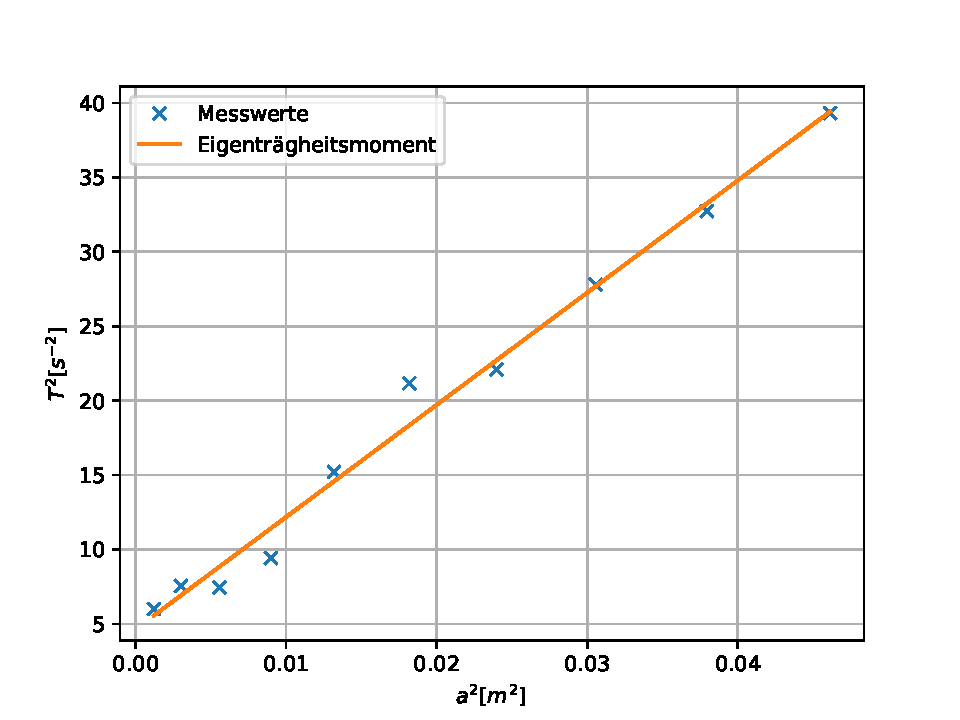
\includegraphics[width=\textwidth]{plotETM.pdf}
  \caption{Messung: Eigenträgheitsmoment}
  \label{fig:linreg}
\end{figure}
\\Die lineare Regression (Abbildung \ref{fig:linreg}) von $T^2$ gegen $a^2$ (Tabelle \ref{tab:ETM}) liefert folgende Parameter
\begin{align*}
  n &= \SI{753.5 \pm 911.8}{\frac{1}{s^2 m^2}}\\
  b &= \SI{4.7 \pm 0.5}{\frac{1}{s^2}}
\end{align*}
\\Formel \eqref{eqn:linb} nach $I_{D}$ umgestellt ergibt
\begin{equation*}
  I_{D} = \frac{b \cdot D}{4 \cdot \pi^2} - 2 \cdot m_{ID} \cdot \left( \frac{r_{ID}^2}{4} + \frac{h_{ID}^2}{12} \right).
\end{equation*}
\\Der Fehler wird mit der Gauß'schen Fehlerfortpflanzung bestimmt
\begin{equation}
  \Delta I_{D} = \sqrt{ \left(\frac{b}{4 \cdot \pi^2}\right)^2 \cdot (\Delta D)^2 + \left(\frac{D}{4 \cdot \pi^2}\right)^2 \cdot (\Delta b)^2}.
\label{eqn:gaussID}
\end{equation}
\\Somit beläuft sich das Eigenträgheitsmoment der Drillachse $I_{D}$ auf
\begin{equation*}
  I_{D} = \SI{-0.0011 \pm 0.0003}{kg m^2}
\end{equation*}
\\Da ein negatives Trägheitsmoment physikalisch nicht möglich ist, wird davon ausgegangen, dass das Eigenträgheitsmoment der Drillachse vernachlässigbar klein ist.


\subsection{Trägheitsmoment des ersten Körpers}


\subsubsection{Theoretische Werte}
Der Radius des vorliegenden Zylinders ist $r_{K1}=\SI{0.0375}{m}$, die Höhe des Zylinders liegt bei $h_{K1}=\SI{0.0299}{m}$ und die Masse wird als $m_{K1}=\SI{1.1182}{kg}$ abgewogen.
Nach Formel \eqref{eqn:Zl} wird ein Trägheitsmoment von\\
\begin{equation*}
  I_{Theo, P1}= \SI{4.8e-04}{kg m^2}
\end{equation*}
\\ermittelt.

\subsubsection{Experimentelle Werte}
Der Körper wird auf der Drillachse um einen Winkel $\phi_{K1}=180°$ ausgelenkt.
Die gemessenen Schwingungsdauern $T_{K1}$ sind in Tabelle \ref{tab:körper1} zu finden und werden gemittelt.
\begin{table}[h!]
  \centering
  \caption{Messdaten der Schwingungsdauern des ersten Körpers}
  \label{tab:körper1}
  \begin{tabular}{c}
    \toprule
     $T_{K1}/\frac{\symup{1}}{\symup{s}}$\\
    \midrule
      \input{Körper1.txt}
    \bottomrule
  \end{tabular}
\end{table}

\\Der Mittelwert der Schwingungsdauern berechnet sich über Formel \eqref{eqn:mw}.
\\Die Standardabweichung wird mithilfe von Formel \eqref{eqn:sigma} ermittelt.
\\Mit fünf Werten errechnet sich der verwendete Wert der Schwingungsdauer zu:
\begin{equation*}
  T_{K1}=\SI{0.857 \pm 0.005}{\frac{\symup{1}}{\symup{s}}}.
\end{equation*}
\\Das Trägheitsmoment wird nach Formel \eqref{eqn:schwing2} berechnet.
Der Fehler für das Trägheitsmoment berechnet sich mithilfe der Gauß'schen Fehlerfortpflanzung:
\begin{equation}
  \Delta I_{Ki}= \sqrt{ \left(\frac{2 \cdot D \cdot T_{Ki}}{4 \cdot \pi}\right)^2 \cdot (\Delta T_{Ki})^2 + \left(\frac{T_{Ki}^2}{4 \cdot \pi}\right)^2 \cdot (\Delta D)^2 }
\label{eqn:gaussk}
\end{equation}
\\Es ergibt sich
\begin{equation*}
  I_{K1}= (\num{2.0} \pm \num{0.2}) \num{e-5} \si{kg m^2}.
\end{equation*}

\subsection{Trägheitsmoment des zweiten Körpers}

\subsubsection{Theoretische Werte}
Der zweite Körpers hat den Radius $r_{K2}= \SI{0.03745}{m}$,  die Höhe $h_{K2}= \SI{0.030}{m}$ und die Masse $m_{K2}= \SI{1.1194}{kg}$.
Das errechnete Trägheitsmoment des Körpers nach der Formel \eqref{eqn:Zs} beläuft sich auf
\begin{equation*}
  I_{Theo, K2}= \SI{7.9e-4}{kg m^2}.
\end{equation*}

\subsubsection{Experimentelle Werte}
Die Messung wird mit einem Auslenkwinkel von $\phi=180°$ ausgeführt.
Die gemessenen Schwingungsdauern sind in Tabelle \ref{tab:körper2} zu finden.
\begin{table}[h!]
  \centering
  \caption{Messdaten der Schwingungsdauer des zweitem Körpers}
  \label{tab:körper2}
  \begin{tabular}{c}
    \toprule
     $T_{K2}/\si{\frac{1}{s}}$\\
    \midrule
      \input{Körper2.txt}
    \bottomrule
  \end{tabular}
\end{table}

Der Mittelwert der Schwingungsdauern wird über Formel \eqref{eqn:mw} berechnet.
\\Die Standardabweichung wird über Formel \eqref{eqn:sigma} berechtet.
\\Der hiermit berechnete Wert für die Schwingungsdauer beläuft sich auf
\begin{equation*}
  T_{K2}=\SI{1.172 \pm 0.013}{\frac{1}{s}}.
\end{equation*}
\\Das Trägheitsmoment errechnet sich mit Formel \eqref{eqn:schwing2}.
\\Der Fehler wird über die Gauß'sche Fehlerfortpflanzung nach Formel \eqref{eqn:gaussk} angegeben.
\\Daraus folgt
\begin{equation*}
  I_{K2}= \SI{3.8 \pm 0.4} 10^{-5} \si{kg m^2}.
\end{equation*}


\subsection{Abmessungen der Puppe}
Die Puppe hat eine Masse von $m_{P}=\SI{0.1628}{kg}$.
Die Radien der Puppe sind in der Tabelle \ref{tab:radienpuppe} aufgetragen.
Die Radien werden jeweils für die einzelnen Körperteile gemittelt.
\begin{table}[h!]
  \centering
  \caption{Abmessungen der Puppe}
  \label{tab:radienpuppe}
  \begin{tabular}{c c c c}
    \toprule
     $r_{Rumpf}/m  $ & $r_{Arm}/m  $ & $r_{Bein}/m  $ & $r_{Kopf}/m  $\\
    \midrule
      \input{maße.txt}
    \bottomrule
  \end{tabular}
\end{table}

Die Mittelwerte der Radien berechnen sich jeweils über Formel \eqref{eqn:mw}.
Die zugehörigen Standardabweichungen errechnen sich mithilfe von Formel \eqref{eqn:sigma}.
Daraus ergeben sich die verwendeten Radien
\begin{align*}
r_{\text{Rumpf}} &= \SI{0.0352 \pm 0.0022}{m} \\
r_{\text{Arm}} &= \SI{0.0136 \pm 0.0007}{m}  \\
r_{\text{Bein}} &= \SI{0.0150 \pm 0.0010}{m} \\
r_{\text{Kopf}} &= \SI{0.0267 \pm 0.0016}{m}.\\
\end{align*}
\\Die Längen der einzelnen Körperteile werden als
\begin{align*}
L_{\text{Rumpf}} &= \SI{0.0924}{m}   \\
L_{\text{Arm}} &= \SI{0.1123}{m}     \\
L_{\text{Bein}} &= \SI{0.1488}{m}    \\
L_{\text{Kopf}} &= \SI{0.045}{m}
\end{align*}
\\abgemessen.
\\Für das Gesamtvolumen werden die Teilvolumina ausgerechnet und addiert.
Alle Körperteile werden als Zylinder genähert.
\\Das Volumen eines Zylinders berechnet sich allgemein mit
\begin{equation}
  V_{Zyl.}= \pi \cdot r^2 \cdot L,
\label{eqn:ZylVol}
\end{equation}
\\wobei L die Länge des Zylinders ist und r der Radius.
\\Mit Formel \eqref{eqn:ZylVol} ergibt sich für die einzelnen Körperteile das Volumen.
Der Fehler wird jeweils über die Gauß'sche Fehlerfortpflanzung berechnet:
\begin{equation}
  \Delta V_{\text{Körperteil}} = \sqrt{ (2 \cdot \pi \cdot L_{\text{Körperteil}} \cdot r_{\text{Körperteil}})^2 \cdot (\Delta r_{\text{Körperteil}})^2 }.
\label{eqn:gaussvol}
\end{equation}
\\Damit ergeben sich die Teilvolumina
\begin{align*}
V_{\text{Rumpf}} &= \SI{0.00036 \pm 0.00004}{m^3} \\
V_{\text{Arm}} &= \SI{6.4895 \pm 0.6890e-5}{m^3} \\
V_{\text{Bein}} &= \SI{0.0001 \pm 0.00001}{m^3} \\
V_{\text{Kopf}} &= \SI{0.0001 \pm 0.00001}{m^3}.
\end{align*}
\\Der Fehler des Gesamtvolumens berechnet sich über die Gauß'sche Fehlerfortpflanzung
\begin{equation*}
  \Delta V_{\text{ges}}= \sqrt{(\Delta V_{\text{Rumpf}})^2 + 4 \cdot (\Delta V_{\text{Arm}})^2 + 4 \cdot (\Delta V_{\text{Bein}})^2 + (\Delta V_{\text{Kopf}})^2 }.
\label{eqn:gaussgvol}
\end{equation*}
\\Das Gesamtvolumen bestehend aus Rumpf, Kopf und je zwei Armen und Beinen beläuft sich also auf
\begin{equation*}
  V_{\text{ges}}= \SI{0.0008 \pm 0.00006}{m^3}.
\end{equation*}
\\Nun werden die Anteile der Teilvolumina am Gesamtvolumen bestimmt:
\begin{equation}
  A_{\text{Körperteil}} = \frac{V_{\text{Körperteil}}}{V_{\text{ges}}}.
  \label{eqn:anteile}
\end{equation}
\\Die Fehler werden über die Gauß'sche Fehlerfortpflanzung berechnet:
\begin{equation}
  \Delta A_{\text{Körperteil}}=
  \sqrt{ \left(\frac{1}{  V_{\text{ges}}  }\right)^2 \cdot (\Delta V_{  {\text{Körperteil}}})^2
   + \left(- \frac{V_{\text{Körperteil}}}{V_{\text{ges}}^2}\right)^2 \cdot (\Delta V_{\text{ges}})^2 }
  \label{eqn:gaussanteile}
\end{equation}
\\Damit ergeben sich folgende Anteile am Gesamtvolumen:
\begin{align*}
A_{\text{Rumpf}} &= \SI{0.45   \pm 0.06}{} \\
A_{\text{Arm}} &=   \SI{0.0812 \pm 0.0103}{} \\
A_{\text{Bein}} &=  \SI{0.13   \pm 0.02}{} \\
A_{\text{Kopf}} &=  \SI{0.126  \pm 0.018}{}.
\end{align*}
\\Aus dem Anteil am Gesamtvolumen wird der Anteil der Gesamtmasse eines Körperteils bestimmt, um die Masse der einzelnen Körperteile zu erhalten.
\\Aus
\begin{equation*}
  m_{\text{Körperteil}}= A_{\text{Körperteil}} \cdot m_{\text{Puppe}}
\end{equation*}
\\ergibt sich:
\begin{align*}
m_{\text{Rumpf}}= \SI{0.0733 \pm 0.0104}{kg} \\
m_{\text{Arm}}= \SI{0.0132 \pm 0.0017}{kg}   \\
m_{\text{Bein}}= \SI{0.021 \pm 0.003}{kg}  \\
m_{\text{Kopf}}= \SI{0.021 \pm 0.003}{kg}.
\end{align*}

\subsection{Trägheitsmoment der Puppe, erste Körperhaltung}

\subsubsection{Theoretische Werte}
Die Trägheitsmomente des Rumpfes und des Kopfes werden durch Formel \eqref{eqn:Zs} errechnet.
Aus dem Satz von Steiner (Formel \eqref{eqn:steiner}) und Formel \eqref{eqn:Zs} folgen die Formeln für die Trägheitsmomente der Arme und Beine:
\begin{equation*}
  I_{\text{Arm}}= \frac{m_{\text{Arm}} \cdot r_{\text{Arm}}^2}{2} + m_{\text{Arm}}(r_{\text{Rumpf}} + r_{\text{Arm}})^2
\end{equation*}
\begin{equation}
  I_{\text{Bein}}= \frac{m_{\text{Bein}} \cdot r_{\text{Bein}}^2}{2} + m_{\text{Bein}} \cdot r_{\text{Bein}}^2
  \label{eqn:bein}
\end{equation}
\\Die Fehler des Trägheitsmoments des Rumpfes und des Kopfes werden mittels folgender Gauß'scher Fehlerfortpflanzung berechnet:
\begin{equation}
  \Delta I_{\text{Körperteil}} = \sqrt{ (m_{\text{Körperteil}} \cdot r_{\text{Körperteil}})^2 \cdot (\Delta r_{\text{Körperteil}})^2 }
  \label{eqn:deltairumpf}
\end{equation}
\\Der Fehler des Trägheitsmoment eines Arms und eines Beins wird über
\begin{equation*}
  \Delta I_{\text{Arm}} = \sqrt{ \left(m_{\text{Arm}}(2 r_{\text{Arm}} + 3 r_{\text{Rumpf}}) \right)^2 \cdot (\Delta r_{\text{Arm}})^2}
\end{equation*}
\begin{equation}
  \Delta I_{\text{Bein}} = \sqrt{ \left(m_{\text{Bein}} \cdot r_{\text{Bein}} (1 + r_{\text{Bein}}) \right)^2 \cdot (\Delta r_{\text{Bein}})^2}
  \label{eqn:ibein}
\end{equation}
\\ermittelt.
\\Der Fehler des Gesamtträgheitsmoments errechnet sich über:
\begin{equation}
  \Delta I_{\text{Theo, Pi}} = \sqrt{ (\Delta I_{\text{Rumpf}})^2 + 4(\Delta I_{\text{Arm}})^2 + 4(\Delta I_{\text{Bein}})^2 + (\Delta I_{\text{Kopf}})^2}
  \label{eqn:deltatheo}
\end{equation}
\\Das Gesamtträgheitsmoment der insgesamt sechs Körperteile ergibt sich durch:
\begin{equation*}
  I_{\text{Theo, P1}}=\SI{7.4 \pm 0.9e-5}{kg m^2}.
\end{equation*}

\subsubsection{Experimentelle Werte}
Die Puppe wird in der ersten Körperhaltung um den Winkel $\phi=90°$ ausgelenkt.
Die Schwingungsdauern werden gemessen und gemittelt (Tabelle \ref{tab:puppe1}).
\begin{table}[h]
  \centering
  \caption{Messdaten der Schwingungsdauern der Puppe, erste Körperhaltung}
  \label{tab:puppe1}
  \begin{tabular}{c}
    \toprule
     $T_{P1}/\si{\frac{1}{s}}$\\
    \midrule
      \input{Puppe1.txt}
    \bottomrule
  \end{tabular}
\end{table}

Der Mittelwert und die Standardabweichung der Schwingungsdauern berechnet sich mithilfe von Formel \eqref{eqn:mw} und Formel \eqref{eqn:sigma}.
\\Die Schwingungsdauer ergibt sich somit zu
\begin{equation*}
  T_{P1}= \SI{0.4 \pm 0.006}{\frac{1}{s}}.
\end{equation*}
\\Über Formel \eqref{eqn:schwing2} wird das Trägheitsmoment berechnet.
\\Der Fehler wird durch die Gauß'sche Fehlerfortpflanzung nach Formel \eqref{eqn:gaussk} bestimmt.
\\Damit berechnet sich
\begin{equation*}
  I_{P1}= \SI{4.7 \pm  0.4} \cdot10^{-6} \si{kg m^2}.
\end{equation*}


\subsection{Trägheitsmoment der Puppe, zweite Körperhaltung}

\subsubsection{Theoretische Werte}
Die Trägheitsmomente der einzelnen Körperteile berechnen sich wie folgt.
Das Trägheitsmoment eines Armes wird aus dem Satz von Steiner (Formel \eqref{eqn:steiner}) und Formel \eqref{eqn:stab} hergeleitet:
\begin{equation*}
  I_{\text{Arm}}= \frac{m_{\text{Arm}} \cdot L_{\text{Arm}}^2}{3} + m_{\text{Arm}} \cdot r_{\text{Rumpf}}^2.
\end{equation*}
\\Die Trägheitsmomente des Rumpfes und des Kopfes werden mit Formel \eqref{eqn:Zs} berechnet.
Das Trägheitsmoment eines Beines wird über Formel \eqref{eqn:bein} ermittelt.
Die Fehler der einzelnen Trägheitsmomente der Körperteile werden durch Formel \eqref{eqn:deltairumpf} und Formel \eqref{eqn:ibein} bestimmt.
Der Fehler des Trägheitsmoments eines Arms errechnet sich durch
\begin{equation*}
  \Delta I_{\text{Arm}}= \sqrt{ \left( 2m_{\text{Arm}} \cdot r_{\text{Rumpf}} \right) \cdot (\Delta r_{\text{Rumpf}})^2 }
\end{equation*}
\\Daraus ergibt sich ein Gesamtträgheitsmoment von
\begin{equation*}
  I_{\text{Theo, P2}}= \SI{0.00018 \pm 0.00002}{kg m^2}.
\end{equation*}
\\Der Fehler wird nach Formel \eqref{eqn:deltatheo} bestimmt.

\subsubsection{Experimentelle Werte}
Für das Trägheitsmoment der Puppe mit der zweiten Körperhaltung wird sie um den Winkel $\phi=90°$ ausgelenkt.
Die Schwingungsdauern werden gemessen und gemittelt (Tabelle \ref{tab:puppe2}).
\begin{table}[h!]
  \centering
  \caption{Messdaten der Schwingungsdauern der Puppe, zweite Körperhaltung}
  \label{tab:puppe2}
  \begin{tabular}{c}
    \toprule
     $T_{P2}/\si{\frac{1}{s}}$\\
    \midrule
      \input{Puppe2.txt}
    \bottomrule
  \end{tabular}
\end{table}

Der Mittelwert der Schwingungsdauern berechnet sich mithilfe von Formel \eqref{eqn:mw}.
Die Standardabweichung wird mit Formel \eqref{eqn:sigma} errechnet.
\\Damit ist die verwendete Schwingungsdauer für die zweite Körperhaltung der Puppe
\begin{equation*}
  T_{P2}= \SI{0.646 \pm 0.012}{\frac{1}{s}}.
\end{equation*}
\\Das Trägheitsmoment berechnet sich mit Formel \eqref{eqn:schwing2}.
\\Der Fehler wird über Formel \eqref{eqn:gaussk} berechnet.
\\Damit berechnet sich das Trägheitsmoment der Puppe in der zweiten Körperhaltung zu
\begin{equation*}
  I_{P2}= \SI{1.158 \pm 0.112} \cdot 10^{-5} \si{kg m^2}.
\end{equation*}
